% !TeX spellcheck = cs_CZ

\documentclass[a4paper]{article}
\usepackage[english]{babel}
\usepackage[utf8x]{inputenc}
\usepackage[T1]{fontenc}
\usepackage{listings}
\usepackage[a4paper,margin=2cm]{geometry}
\usepackage{amsmath}
\usepackage{graphicx}
\usepackage[colorinlistoftodos]{todonotes}
\usepackage[colorlinks=true, allcolors=blue]{hyperref}
\usepackage{wasysym} % smileys
\usepackage{fancyhdr}
\setlength\parindent{0pt} % indent

% my commands:
\newcommand{\n}{\newline}
\newcommand{\tab}{\hspace{1cm}}

\begin{document}

\thispagestyle{fancy} % beware the difference between \thispagestyle and \pagestyle
\lhead{1. Domácí úkol}
\rhead{Vilém Zouhar}

\section{}
% PROGRESS 1
\subsection{}
Zadání interpretuji tak, že si každý kamarády vybírá náhodný zákusek, nikoliv náhodný druh.
Spočítáme počet příznivých výsledků kýženého jevu a pak celkový počet. Podmínku splníme tak, že první tři lidé si vezmou od každého jeden a pak zbytek libovolné různé. Jsou to jevy disjunktní, takže vynásobíme třemi. Celkový počet výsledků je jednoduše výběr z $9$ zákusků $5$ lidmi.
\begin{align*}
	P = \frac{3 \cdot {6 \choose 2}}{{9 \choose 5}} = \frac{5}{14}	
\end{align*}

% PROGRESS 1
\subsection{}
Z každého druhu si musí vzít lidé dohromady 2.
\begin{align*}
	P = \frac{{3 \choose 2}^3}{{9 \choose 6}} = \frac{9}{28} \\	
\end{align*}
Jinou úvahou můžeme spočítat opačný jev (zaplníme alespoň jeden ze zákusků)
\begin{align*}
	P = 1-\frac{3 \cdot ({6 \choose 3}-2 )+3}{{ 9 \choose 6}} = 1 - \frac{19}{28}
\end{align*}

% PROGRESS 1
\subsection{}
Jestliže zůstal jen jeden věneček, tak zbyly i zároveň i 3 další zákusky. Pokud si tedy Adam vybere, tak si musí vzít jeden z těch tří, aby zůstal věneček. Jelikož si vybírá náhodně uniformně, tak triviálně je z toho pravděpodobnost $\frac{3}{4}$.

\newpage
\section{}
% PROGRESS 1
\subsection{}
Marginální rozdělení nalezneme v posledním sloupci/posledním řádku. Sdružené rozdělení je popsáno vevnitř.
\begin{center}
\begin{tabular}{| c | c | c | c | c | }\hline
	$X\backslash Y$ & 0 & 1 & 2 & \\ \hline
	0 & $\frac{105}{248}$ & $\frac{63}{496}$ & $\frac{3}{496}$ & $\frac{69}{124}$ \\ \hline
	1 & $\frac{147}{496}$ & $\frac{21}{248}$ & $\frac{3}{496}$ & $\frac{12}{31}$ \\ \hline
	2 & $\frac{21}{496}$  & $\frac{7}{496}$  & $0$ 			   & $\frac{7}{124}$\\ \hline
	  & $\frac{189}{248}$ & $\frac{7}{31}$ 	 & $\frac{3}{248}$ & 1\\ \hline
\end{tabular}
\end{center}

% PROGRESS 1
\subsection{}
\begin{align*}
	& E[X] = \frac{12}{31} + \frac{2\cdot 7}{124} = \frac{1}{2} \\
	& E[Y] = \frac{7}{31} + \frac{2\cdot 3}{248} = \frac{1}{4} \\
	& E[XY] = \frac{21}{248} \cdot 1 \cdot 1 + \frac{3}{496} \cdot 1 \cdot 2 + \frac{7}{496} \cdot 1 \cdot 2 = \frac{1}{8} \\
	& cov(X,Y) = E[XY] - E[X]E[Y] = 0 \Rightarrow corr(X,Y) = 0 \\ 
	& P[X=2] \ne 0, P[Y=2] \ne 0, P[X=2,Y=2] = 0 \ne P[X]P[Y] \Rightarrow P[XY] \ne P[X]P[Y] \Rightarrow \text{ závislé}
\end{align*}

\subsection{}
\begin{center}
\begin{tabular}{| c | c | }\hline
	  & $Z^a$  \\ \hline
	0 & $\frac{(24-a)(23-a)}{552}$  \\ \hline
	1 & $\frac{a(24-a)}{276}$  \\ \hline
	2 & $\frac{a\cdot(a-1)}{552}$  \\ \hline
\end{tabular}
\end{center}

\begin{align*}
	& P[a = i] = \frac{{8 \choose i}\cdot {24 \choose 8-i}}{{32 \choose 8}} \\	
	& E[Z^a] = P[Z^a=1] + 2\cdot P[Z^a = 2] =  \frac{a(24-a)}{276} + 2\cdot \frac{a\cdot(a-1)}{552}= \frac{a}{12}
\end{align*}

% PROGRESS 1
\subsection{}
Máme zajištěný nestranný odhad střední hodnoty:
\begin{align*}
	& \frac{1}{n} \sum Z_i = \widehat{EZ} = \frac{a}{12} \Rightarrow \hat{a} = 12\cdot \widehat{EZ} \\
	% & \text{(Zaokrouhlujeme nahoru, protože pokud vytáhneme alespoň jednu srdcovou kartu, pak jistě $a \ne 0$.)}
\end{align*}

Zaokrouhlujeme nahoru, neboť pokud dostaneme alespoň jednu nenulovou $Z_i$, pak rozhodně $a \ne 0$.

% PROGRESS 1
\subsection{}
Provedeno 10000 takových pokusů (pro $n=20$). Průměrný součet rozdílů reálné a odhadované hodnoty vyšel $-0.004298$, což je číslo blízko nuly a naznačuje to, že odhad je nestranný. (viz. kód)


\newpage 
\section{}
% PROGRESS 1
\subsection{}
\begin{align*}
	F(a) = \int_1^a \frac{2}{x^3} dx = \big[\frac{-1}{x^2}\big]_1^a = 1 - \frac{1}{a^2} \\
	P[x \le 5] = F(5) = 1- \frac{1}{25} = \frac{24}{25}
\end{align*}

\begin{center}
	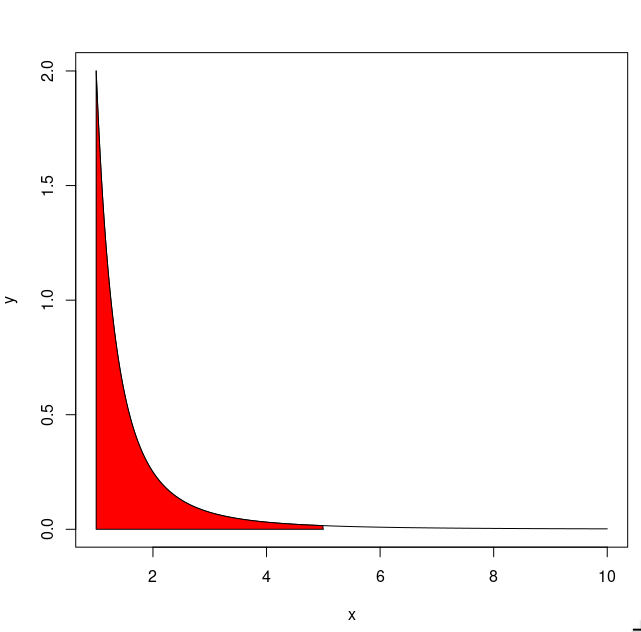
\includegraphics[width=0.6\textwidth]{density}
\end{center}
Jedná se o plochu grafu pod křivkou pro $f(x), x \le 5$

% PROGRESS 1
\subsection{}
\begin{align*}
	E[X] = \int_1^\infty x \cdot \frac{2}{x^3} dx = \int_1^\infty \frac{2}{x^2} dx = \big[\frac{-2}{x}\big]_1^\infty = 2
\end{align*}

% PROGRESS 1
\subsection{}
\begin{align*}
	& E[X^2] = \int_1^\infty x^2 \cdot \frac{2}{x^3} dx = [2\ln(x)]_1^\infty = \infty, E[X] \ne \infty \Rightarrow var(X) = \infty
\end{align*}

% PROGRESS 1
\subsection{}
\begin{align*}
	& f_U = \begin{cases} 1 \tab 0 \le x \le 1 \\ 0 \tab otherwise \end{cases} \\
	& F_U = \begin{cases} 0 \tab x < 0 \\ x \tab x \in (0, 1) \\ 1 \tab x \ge 1 \end{cases} \\
	& X = 1-\frac{1}{U^2} \rightarrow F_X(u) = P[1-\frac{1}{U^2} \le u] = P[1-u \le \frac{1}{U^2}] = P[U^2 \le \frac{1}{1-u}] = P\bigg[U \le \frac{\pm 1}{\sqrt{1-u}} \bigg] = F_U \bigg(\frac{\pm 1}{\sqrt{1-u}}  \bigg) \\
	& \text{Volíme znamínko +, neboť tak jedině bude dávat výraz smysl. Pro dané $u$ bereme: } x = \frac{1}{\sqrt{1-u}}. \\ 
	& \text{Výraz omezujeme pro } u \in (0, 1], \text{ ale to nevadí, neboť } P[u=0] = 0 
\end{align*}

% PROGRESS 0.8
\subsection{}

$mean(X_1, \ldots, X_{20}) \ \text{}\ = 2.53213806654802$ \\
$mean(X_1, \ldots, X_{100}) \ = 1.85682741732373$ \\
$mean(X_1, \ldots, X_{1000}) = 1.95906747082822$ \\

Odhady vypadají konzistentně - se zvyšujícím počtem pokusů se odhad střední hodnoty zlepšuje.

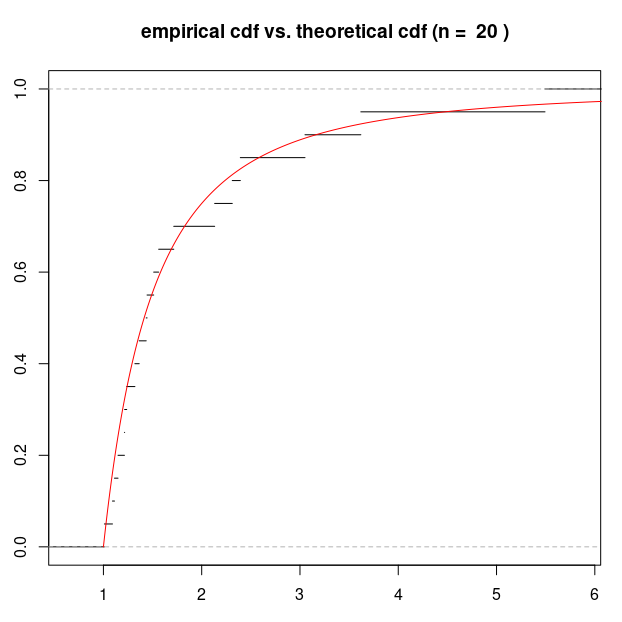
\includegraphics[width=0.5\textwidth]{trial_20}
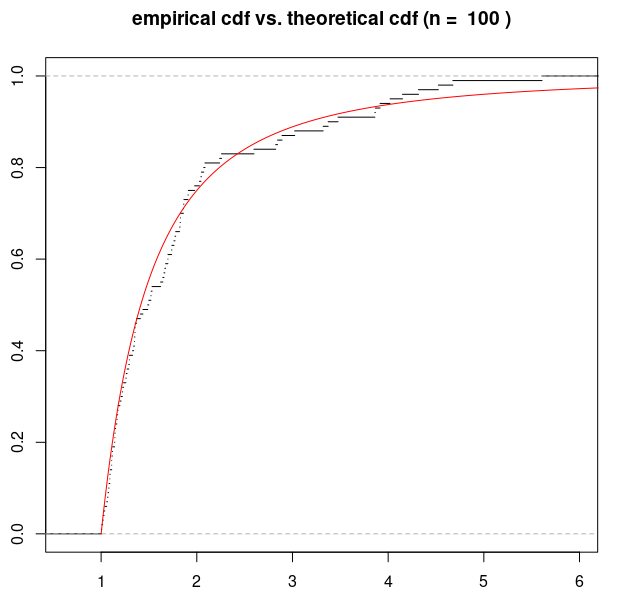
\includegraphics[width=0.5\textwidth]{trial_100}\\
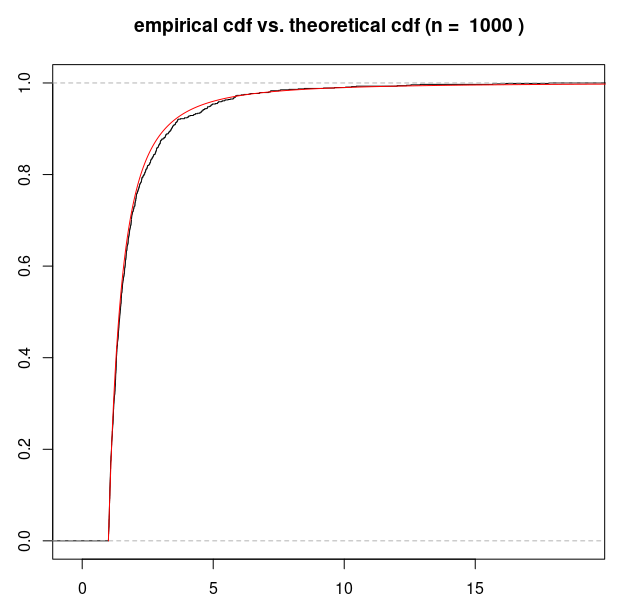
\includegraphics[width=0.7\textwidth]{trial_1000}

\newpage
% PROGRESS 1
\section*{Code}
\begin{lstlisting}
# 2.e
mean(sapply(1:10000, function(i) {
        # 1 - hearts, 0 otherwise
        cards = sample(c(rep(0, 24), rep(1, 8)), 32)[1:24]
        resC = sapply(1:20, function(i) sum(sample(cards, 2)))
        p_a = 12 * mean(resC)
        r_a = sum(cards)
        return(r_a-p_a)
}))

# 3.a
f = function(x) { if(x >= 1) { return(2/x^3);}  else { return(0); } }
F = function(x) { return(1-1/x^2); }

x = seq(1, 20, 0.001)
y = sapply(x, f)
Y = sapply(x, F)

plot(x, y, type='l')
polygon(c(1, x[x<5], 5),  c(0, y[x<5], 0), col="red")

# 3.e
U = function() sample(seq(10^-6, 1, 10^-6), 1)
X = function(u) 1/sqrt(1-u)

trial = function(n) {
        resX = sapply(1:n, function(i) X(U()))
        # drop results > 20, this is not correct, but makes the graph more readable
        resX = resX[resX < 20]
        plot(ecdf(resX), do.points=FALSE,
                main=paste('empirical cdf vs. theoretical cdf (n = ', n, ')'))
        lines(x, Y, type='l', col='red')
        message(n, ' : ',  mean(resX))
}
trial(20)
trial(100)
trial(1000)
\end{lstlisting}
\end{document}